% VUT FIT MITAI
% MSZ 2021/2022
% Author: Vladimir Dusek
% Login: xdusek27

%%%%%%%%%%%%%%%%%%%%%%%%%%%%%%%%%%%%%%%%%%%%%%%%%%%%%%%%%%%%%%%%%%%%%%%%%%%%%%%%

% Path to figures
\graphicspath{{avs/datovy_paralelismus/figures}}

%%%%%%%%%%%%%%%%%%%%%%%%%%%%%%%%%%%%%%%%%%%%%%%%%%%%%%%%%%%%%%%%%%%%%%%%%%%%%%%%

\chapter{AVS~--~Datový paralelismus SIMD, HW implementace a SW podpora.}

%%%%%%%%%%%%%%%%%%%%%%%%%%%%%%%%%%%%%%%%%%%%%%%%%%%%%%%%%%%%%%%%%%%%%%%%%%%%%%%%

\section{Zdroje}

\begin{compactitem}
    \item \path{AVS-05.pdf}
    \item \path{AVS_2019-10-21.mp4}
\end{compactitem}

%%%%%%%%%%%%%%%%%%%%%%%%%%%%%%%%%%%%%%%%%%%%%%%%%%%%%%%%%%%%%%%%%%%%%%%%%%%%%%%%

\section{Paralelismus v procesorech}

\begin{compactitem}
    \item Flynnova taxonomie: \begin{compactitem}
        \item SISD (\textit{single instruction stream, single data stream} -- Skalární procesor.
        \item SIMD (\textit{single instruction stream, multiple data streams} -- Vektorové procesory.
        \item MISD (\textit{multiple instruction streams, single data stream} -- Používá se pouze ve velmi speciálních případech.
        \item MIMD (\textit{multiple instruction streams, multiple data streams} -- Vícevláknové procesory.
    \end{compactitem}

    \begin{figure}[H]
        \centering
        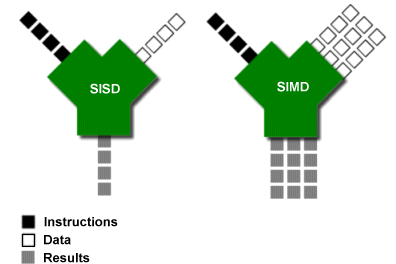
\includegraphics[width=0.6\linewidth]{sisd_simd.png}
        \caption{SISD vs SIMD.}
    \end{figure}

    \item Instrukční paralelismus: \begin{compactitem}
        \item Superskalární procesory -- instrukční paralelismus řízen pomocí hardware (\break OOO, pipeline).
        \item Procesory s dlouhým instrukčním slovem VLIW -- instrukční paralelismus řízen software (kompilátor) nebo hrubé granularitě (vlákna - TLP, procesy).
    \end{compactitem}

    \item Doposud jsme se zabývali instrukčním paralelismem, tedy jak provádět více instrukcí zároveň. Nyní, máme jednu instrukci a ta se aplikuje na více dat (SIMD) $\Rightarrow$ zjednodušení řízení procesoru!
\end{compactitem}

%%%%%%%%%%%%%%%%%%%%%%%%%%%%%%%%%%%%%%%%%%%%%%%%%%%%%%%%%%%%%%%%%%%%%%%%%%%%%%%%

\section{Datový paralelismus v procesorech (SIMD)}

\begin{compactitem}
    \item SIMD architektury obsahují velký počet výpočetních jednotek (PE, processing units) a řídící procesor. \begin{compactitem}
        \item Soubor procesorů řízený centrální jednotkou pracuje synchronně po instrukcích, všechny procesory dělají totéž. Některé procesory mohou stát (NOP). Je nezbytné změnit způsob uvažování, při mapování algoritmů na tyto architektury. V současnosti
        \item Implementováno pomocí AVX/SSE registrů.
    \end{compactitem}

    \item Nejsou považovány za univerzální výpočetní systémy; pro
    některé testy špičková výkonnost, pro jiné jen nízká. \begin{compactitem}
        \item Používají se jako HW akcelerátory a koprocesory (GPU, AVX).
        \item Silná stránka: práce s vektory, maticemi (zvuk, video, diferenciální rovnice, neuronové sítě, \ldots)
        \item Slabá stránka: podmíněné příkazy, switch.
    \end{compactitem}

    \item Výpočet jednotlivých prvků musí probíhat nezávisle na
    ostatních.

    \item Kdy má smysl přemýšlet nad SIMD (vektorizací) \begin{compactitem}
        \item Propustnost paměti -- stíhám procesoru předávat data?
        \item Výkon -- mám dost výkonu abych spočítal data, která mám v procesoru?
    \end{compactitem}
\end{compactitem}

\subsection{Architektury se sdílenou pamětí}

\begin{compactitem}
    \item Paměťové moduly sdíleny všemi PE elementy.
    \item Čtení i zápis dat probíhá skrze dynamickou propojovací síť (např. křížový přepínač).
    \item Jednotlivé PE elementy komunikují pouze přes sdílenou paměť.
    \item Současné architektury GPU se nejvíce podobají tomuto modelu.

    \begin{figure}[H]
        \centering
        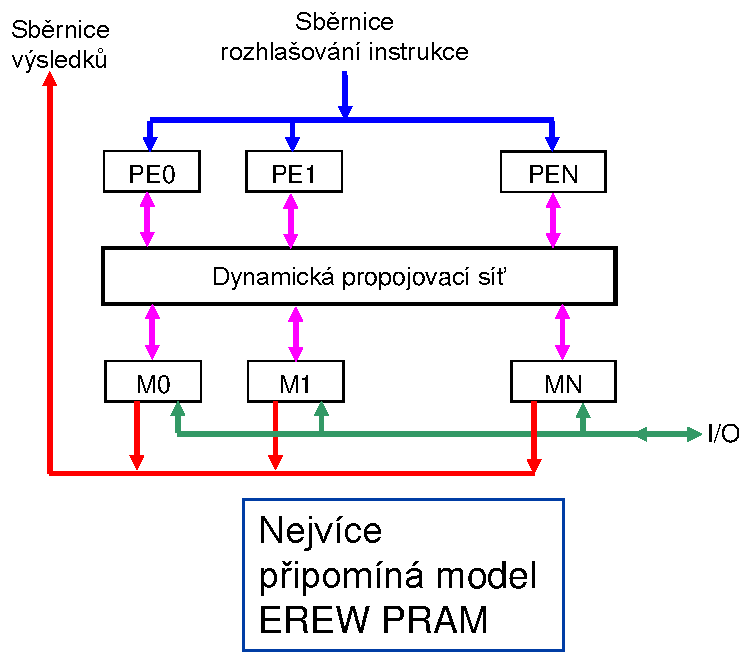
\includegraphics[width=0.75\linewidth]{simd_sdilena.pdf}
        \caption{SIMD se sdílenou pamětí.}
    \end{figure}
\end{compactitem}

\subsection{Architektury s distribuovanou pamětí}

\begin{compactitem}
    \item Každý PE má svůj vlastní paměťový modul -- většinu výpočtu provádí nad lokálními daty.
    \item Komunikace resp. výměna dat s ostatními PE elementy probíhá skrze statickou propojovací síť (např. mřížka, torus, \ldots).

    \begin{figure}[H]
        \centering
        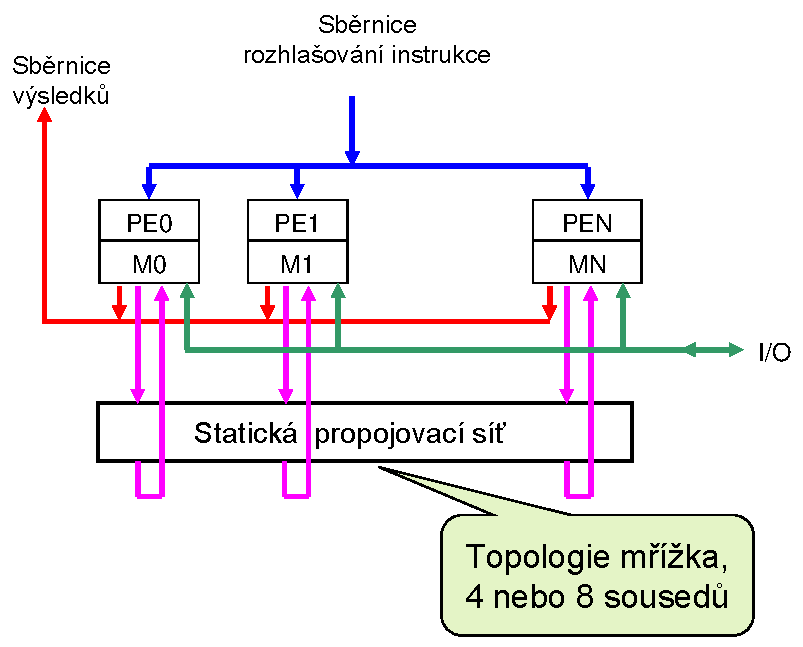
\includegraphics[width=0.75\linewidth]{simd_distribuovana.pdf}
        \caption{SIMD se distribuovanou pamětí.}
    \end{figure}
\end{compactitem}

%%%%%%%%%%%%%%%%%%%%%%%%%%%%%%%%%%%%%%%%%%%%%%%%%%%%%%%%%%%%%%%%%%%%%%%%%%%%%%%%

\section{HW implementace}

\begin{compactitem}
    \item Typicky SWAR (SIMD within a register).

    \item 16 nebo 32 tzv. vektorových registrů o velikosti typicky 512\,bitů.

    \item Každý registr je rozdělen do několika nezávislých částí.

    \item Daná instrukce je vykonána na každé části registru v jednom kroku.

    \item Nejznámější SWAR rozšíření dnešních CPU: AVX, SSE.
\end{compactitem}

%%%%%%%%%%%%%%%%%%%%%%%%%%%%%%%%%%%%%%%%%%%%%%%%%%%%%%%%%%%%%%%%%%%%%%%%%%%%%%%%

\section{SW podpora, vektorizace}

\begin{compactitem}
    \item Jak vektorizovat? \begin{compactitem}
        \item vektorizované knihovny (Intel MKL, Atlas, Numpy, Scipy);
        \item automatické vektorizace kompilátorem (\path{-o3}, \path{-vec});
        \item pragma hints pro kompilátor do zdrojového kódu (OpenMP);
        \item vektorové intrinsic funkce.
    \end{compactitem}

    \begin{figure}[H]
        \centering
        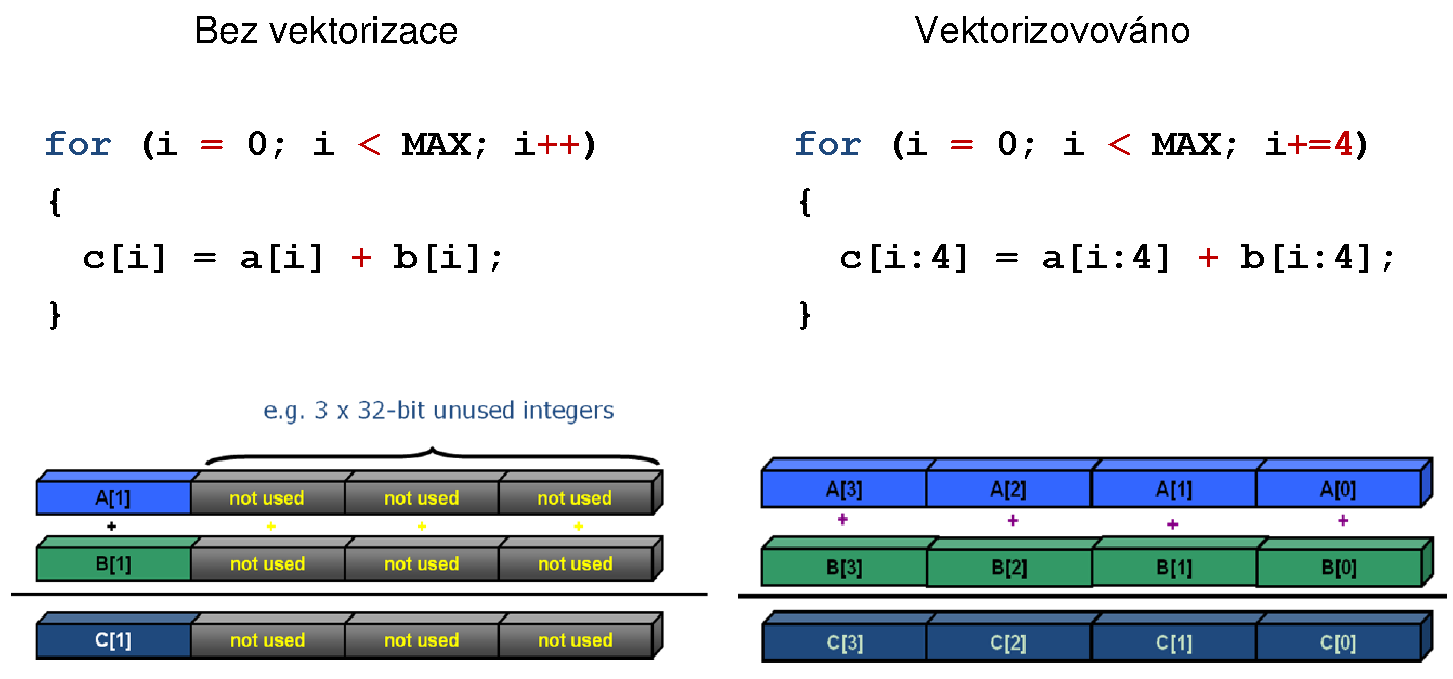
\includegraphics[width=1\linewidth]{vektorizace.pdf}
        \caption{Příklad vektorizace. Načítám naráz 4 prvky, počítám naráz 4 prvky, ukládám naráz 4 prvky.}
    \end{figure}

    \item Co dokáže kompilátor auto vektorizovat? \begin{compactitem}
        \item Cyklus kde známe počet iterací už v době, kdy do něho vstoupíme (v těle cyklu se nemůže měnit podmínka).
        \item Cyklus který má jeden vstup a jeden výstup (žádný breaky a continue).
        \item Cyklus který nemá podmínky a volání funkcí.
        \item V případě vnořených cyklů lze vektorizovat pouze ten nejvnitřnější.

        \begin{figure}[H]
            \centering
            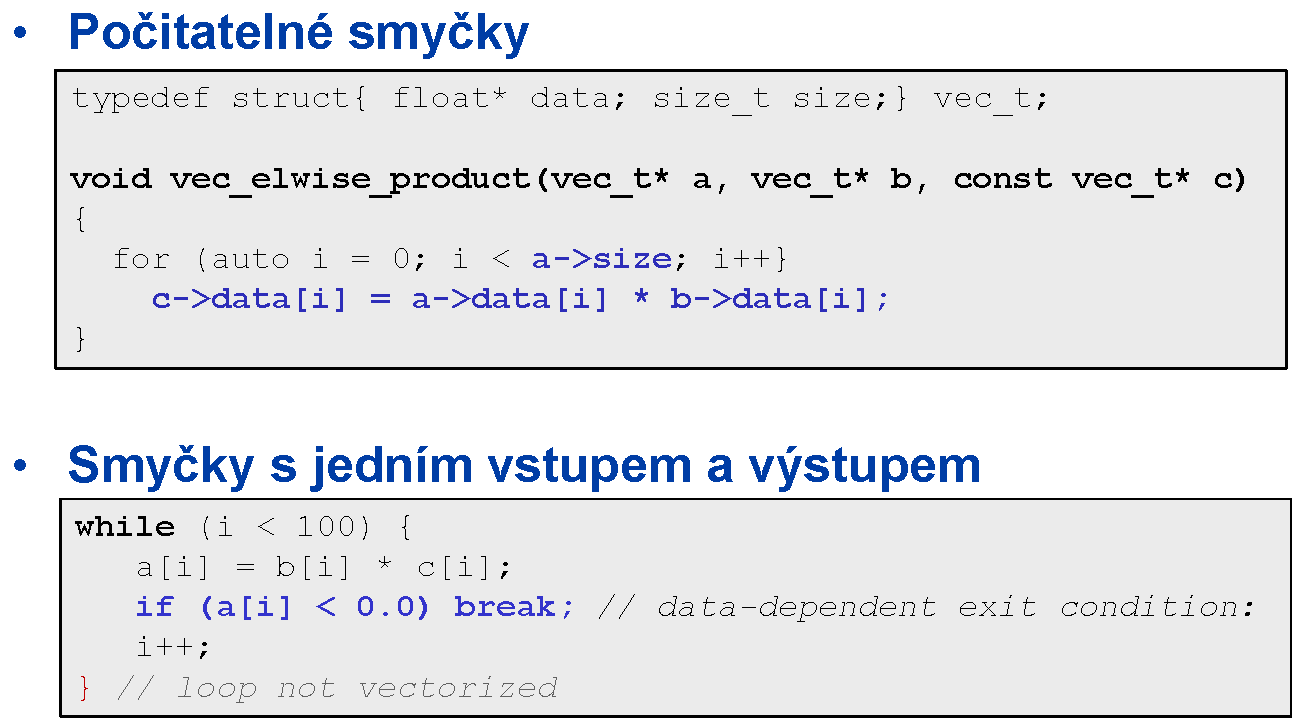
\includegraphics[width=0.85\linewidth]{auto_vektorizace_1.pdf}
            \caption{Příklad toho, co dokáže kompilátor auto vektorizovat.}
        \end{figure}

        \begin{figure}[H]
            \centering
            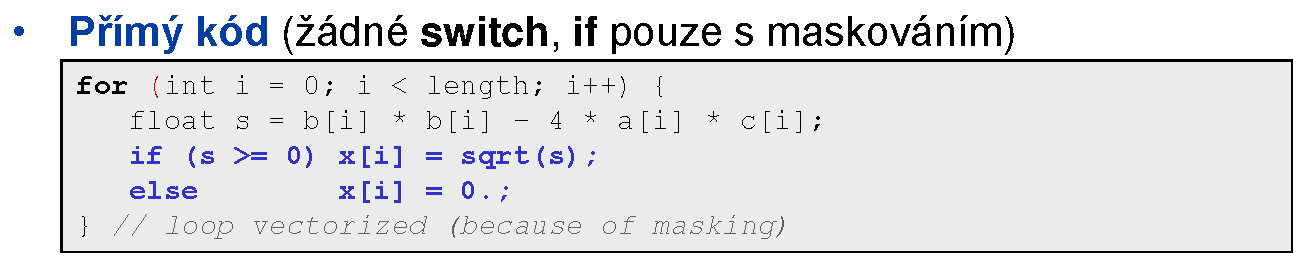
\includegraphics[width=0.85\linewidth]{auto_vektorizace_2.pdf}
            \caption{Příklad toho, co dokáže kompilátor auto vektorizovat.}
        \end{figure}
    \end{compactitem}

    \item Na čem může selhat? \begin{compactitem}
        \item Nejednotkový rozestup: $b[i] + a[i+5]$.
        \item Nezarovnané datové struktury.
        \item Datové závislosti mezi iteracemi -- OpenMP nekontroluje, programátor musí hlídat.
        \item Pointer aliasing (překryté paměťové prostory).
        \item Data musí být zarovnaná na velikosti SIMD registru (16, 32, 64 bytů pro SSE, AVX, AVX-512).
    \end{compactitem}

    \item Datové struktury jsou problém. \begin{compactitem}
        \item Pole struktur vs struktura polí, co je \uv{hezké} z hlediska OOP, může být z hlediska vektorizace problém.
    \end{compactitem}

    \begin{figure}[H]
        \centering
        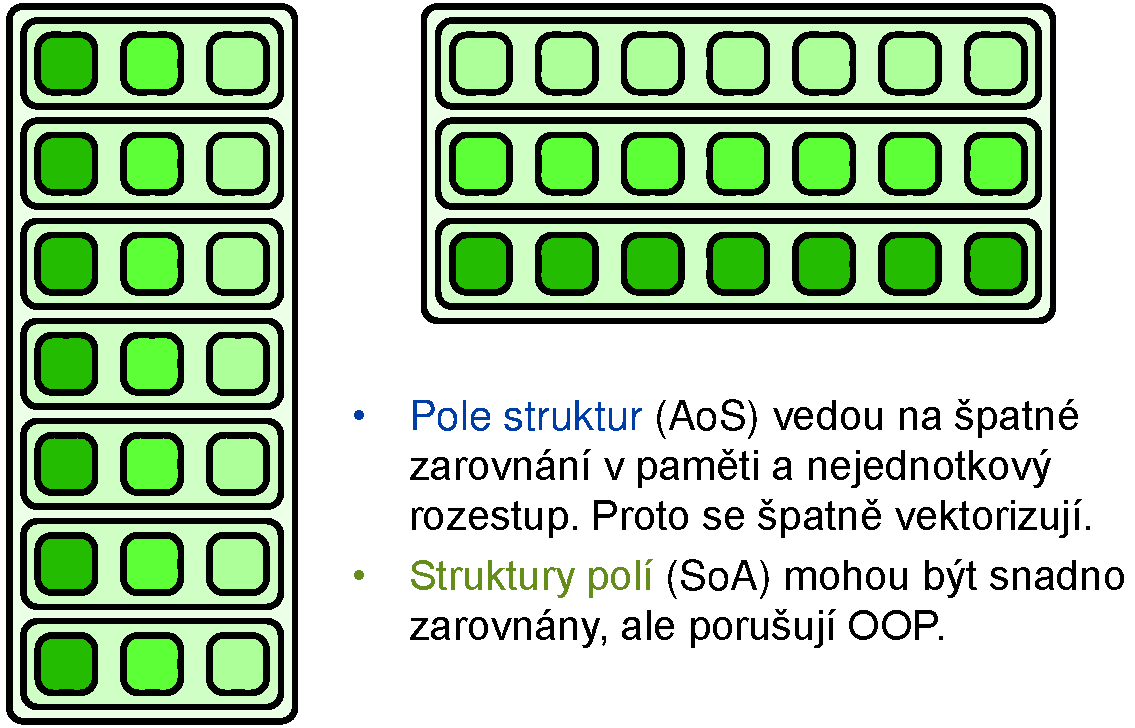
\includegraphics[width=0.85\linewidth]{datove_struktury.pdf}
        \caption{Datové struktury -- AoS nebo SoA.}
    \end{figure}
\end{compactitem}

%%%%%%%%%%%%%%%%%%%%%%%%%%%%%%%%%%%%%%%%%%%%%%%%%%%%%%%%%%%%%%%%%%%%%%%%%%%%%%%%

\section{Vektorizace pomocí OpenMP}

\noindent\begin{minipage}{\linewidth}
\begin{lstlisting}[language=bash, caption={Obyčejná smyčka.}]

void add(float* a, float* b, float* c, float* d, float* e, int n)
{
    #pragma omp simd
    for (int i = 0; i < n; i++) {
        a[i] = a[i] + b[i] + c[i] + d[i] + e[i];
    }
}

\end{lstlisting}
\end{minipage}

\noindent\begin{minipage}{\linewidth}
\begin{lstlisting}[language=bash, caption={Redukce, po skončení vektorovýho výpočtu posčítá mezivýsledky.}]

#pragma omp simd reduction(+:sum)
for (i = 0; i < *p; i++) {
    A[i] = B[i] * C[i];
    sum = sum + A[i];
}

\end{lstlisting}
\end{minipage}

\noindent\begin{minipage}{\linewidth}
\begin{lstlisting}[language=bash, caption={Aligned, dané proměnné jsou zarovnány na počet bytů.}]

#pragma omp simd aligned(sum:64)

\end{lstlisting}
\end{minipage}

\noindent\begin{minipage}{\linewidth}
\begin{lstlisting}[language=bash, caption={Safelen, maximální počet iterací, které se mohou vykonávat současně bez porušení závislostí.}]

#pragma omp simd safelen (10)
for (i = 0; i < MAX; i++) {
    a[i] += a[i - 10]
}

\end{lstlisting}
\end{minipage}

\noindent\begin{minipage}{\linewidth}
\begin{lstlisting}[language=bash, caption={Linear, hodnota proměnné je ve vztahu k číslu iterace.}]

#pragma omp simd linear (x)
for (i = 0; i < MAX; i++) {
    x[i] = x_orig + i * linear_step
}

\end{lstlisting}
\end{minipage}
